\documentclass{jspf}            % プラズマ・核融合学会誌
\usepackage{graphicx}           % 図をインクルードする
\usepackage{amsmath}            % AMS-LaTeXを使う
\usepackage{amssymb}            % TXフォントの場合は不要
%\usepackage{txfonts}           % TXフォント(Times/Helvetica)を使う
%\renewcommand{\ttdefault}{cmtt}% TXフォントの際の等幅フォントの設定
\usepackage{url}                % \url{...}マクロを使う
\usepackage{color}
\usepackage{listings,jlisting}

\newcommand{\wz}{\omega_z}
\newcommand{\vu}{\vec{u}}
\newcommand{\vr}{\vec{r}}
\renewcommand{\div}{\nabla \cdot}

\renewcommand{\vec}[1]{\bm{#1}}

\usepackage{bm}
\usepackage{udline} % \Sl{…}で改行あり打ち消し線

\begin{document}                % 始まり

% 和文タイトル(途中の改行は \\ で)
\title{超並列粒子法シミュレーションプログラム自動生成ツールの紹介\\
〜並列プログラミング初心者にもできる!〜}

% 和文著者
\author{野村昴太郎$^{1,2)}$,沼田龍介,八柳祐一,行方大輔$^{1,2)}$,岩澤全規$^{1,2)}$,牧野淳一郎$^{1,2)}$\\
$^{1)}$神戸大学 惑星科学研究センター\\
$^{2)}$理化学研究所 計算科学研究センター\\
$^{3)}$兵庫県立大学大学院シミュレーション学研究科\\
$^{1)}$静岡大学教育学部\\
}

% 欧文タイトル

\etitle{Introduction to auto-generator tool of massive parallel simulation code.}

% 欧文著者

\eauthor{NOMURA Kentaro$^{1,2)}$, NUMATA Ryusuke$^{3)}$, YATSUYANAGI Yuichi$^{3)}$, \\
NAMEKATA Daisuke$^{1,2)}$, IWASAWA Masaki$^{1,2)}$, MAKINO Junichiro$^{1,2)}$}


% 日付

\date{(原稿受付:2019年??月??日)}

% アブストラクト

\begin{abstract}
本稿では、私達が開発・公開している多体シミュレーション
プログラム開発フレームワーク「FDPS (Framework for Developping Particle
  Simulators)」を紹介します。FDPS は、粒子シミュレーションを研究に使っ
ている多くの研究者が、並列化や計算機アーキテクチャ固有のチューニングに
多大な時間を費やすことなく、自分の扱いたい問題向けのシミュレーションプ
ログラムを容易に作成できるようになることを目標として開発したフレームワー
クです。連載第一回の今回は、FDPS の開発の背景、考え方と、実際にどのよ
うなことができるか、という簡単な例を紹介します。
\end{abstract}

% キーワード

\keywords{FDPS, 粒子系シミュレーション,プラズマシミュレーション}

% 主著者のメールアドレス(_ や % もそのまま書けます)
\AuthorsEmail{kentaro.nomura@riken.jp}
%%%%%%%%%%%%%%%%%%%%%%%%%%%%%%%%%%%%%%%%%%%%%%%
\section{はじめに}
我々が FDPS を開発した動機は、
現在、大規模な粒子シミュレーションを
する、特に、そのためのプログラムを開発することが非常に大変になってい
る、ということです。FDPS はこの開発を容易にすることを目指すものです。

30年前であれば、研究に使える粒子シミュレーションのプログラムを研究者、
あるいは学生が自分で書くことはそれほど大変ではありませんでした。普通に
書いた上で、ベクトル化等をすればよかったからです。

しかし、現在では、そう簡単ではありません。
まず、1CPUの計算機でも、
CPU コアが複数あり、コアの中にはSIMDユニットがあるため、これらを有効に
使えるかどうかで数十から数百倍性能が変わります。また、キャッシュメモリ
も有効に使わない逆に性能が桁で落ちることもあります。さらにスパコンを、
と思うとMPIを使った並列化が必要です。これらをあわせるとそもそも個人で
は困難、というレベルの大変な作業になります。

大変になっている要因を整理してみると、次のようにまとめられます。

\begin{itemize}

\item 並列化の階層の増加

\item メモリボトルネックの発生とそれには対応したメモリ階層の増加・複雑化

  
\end{itemize}  

以下、それぞれについて簡単に述べます。

現代の典型的な大規模並列計算機は、

\begin{itemize}

\item 複数の演算を並列に行う SIMD 演算ユニットを (コア内SIMD)
\item 複数もつ演算コアを (スーパースカラー)
\item 複数もつプロセッサチップを (マルチコア)
\item 複数ネットワークで接続した (分散メモリ並列)

\end{itemize}  
構成を持っています。つまり、4つの違うレベルで並列動作する複数のユニッ
トを持っています。しかも、それぞれのレベルで、どういうふうにすれば上手
く並列化できるか、が違います。この中で、「スーパースカラー」というのは、
CPU が、機械語プログラムの中から、並行して実行できそうなものを同時に
実行する機能です。なので、これは
ある程度ハードウェアがやってくれます。しかし、他の3つのレベルのために固有の
最適化が必要で、しかも分散メモリ並列では MPI を使ってプログラム全体を
書換え、例えば空間分割をして粒子を移動させるといった処理も書く必要がで
てきます。

並列化の複数のレベルの扱いをさらに困難なものにしているのが、メモリ階層
の存在です。現代の計算機では、演算器のほうがメモリより速く、演算器の性能を生
かすためには容量は小さいけれど高速なキャッシュメモリを使っています。

しかし、この、キャッシュメモリは、並列計算機とは決して相性のいいもので
はありません。マルチコアプロセッサでは、それぞれのコアが独立にキャッシュ
をもちたいわけですが、そうすると、あるコアがメモリのどこかに書いても、
その同じアドレスのデータを別のコアが自分のキャッシュにもっているとか、
あるいはまだ誰かのキャッシュの中でしか更新されていなくて主記憶には古い
データがあるものを主記憶から読んだ時に新しいデータにならないといけないといった
問題があります。こういったややこしい状況でもちゃんと整合性がある結果を
保証するのが「コヒーレントキャッシュ」というもので、そのためにコア間で
複雑なやりとりをする大規模なハードウェアが必要です。

このようなシステムで性能を出すためにはいかにしてキャッシュを制
御するかが重要になり、キャッシュの特性を考慮したプログラムを書く必要
がでてきます。最近のプロセッサでは3レベルから4レベルのキャッシュを持つ
ようになっています。しかし、密行列乗算ならともかく、それ以外の計算アル
ゴリズムではこのような複数レベルのキャッシュを有効に使えるとは限らないで
すし、できたとしてもプログラムは極めて複雑なものにならざるを得ません。

このため、単純なアルゴリズムでも、最新の高性能プロ
セッサで性能を出すのは容易なことではなくなっています。

実際、今この文章を読んでおられる読者の皆様の中でも、俺はMPIで並列化し
てキャッシュも有効利用しSIMD演算器も使ってプラズマシミュレーションプロ
グラムを書いた、あるいは書ける、あるいは書く気がある、という人はあまり
多くないのでは、と思います。

では、どうすればいいのか?というのがここでの問題です。多くの場合にとら
れているアプローチは、大規模なソフトウェアを開発チームを作ることでなん
とか開発しよう、というもので、実際、様々な応用分野で、粒子法の並列化さ
れたプログラムが公開され、利用可能になっています。

しかし、そういったプログラムは、あらかじめ開発グループが実装した機能を、
開発グループがターゲットにしたマシン・OSで使うことしかできないのが普通
です。もちろん、オープンソースで公開されているものでは、原理的には
ソースコードを修正していろいろな機能を実装できるわけですが、巨大で複雑
なプログラムで、さらに特定のアーキテクチャ向けの最適化されたコードがで
るものを修正して動くようにするのは容易なことではないのは、やってみよう
と思ったことがある人は良くご存じのことかと思います。

なので、自分でプログラムを開発できるようにしたいわけですが、それにはど
うすればいいのか、というのが我々の問題意識です。我々が提案する方法は、
特にMPIにかかわるような複雑な並列化とそのために必要なプログラムと、実
際に扱う系の記述や時間積分の方法の記述とを明確に分離することです。

明確に分離、と書くのは簡単ですが、実際にどのように実現するか、
十分に色々なことを表現するにはどうするか、計算速度がでるようにするには
どうするのか、と、いろいろな問題があります。本解説では、まず
基本的な考え方を2節で、またいくつかのFDPSをつかったサンプルを3節で紹
介します。4節はまとめです。

%%%%%%%%%%%%%%%%%%%%%%%%%%%%%%%%%%%%%%%%%%%%%%%
\section{FDPSの基本的な考え方}

大規模並列化が可能で実行性能も高いMPI並列化粒子法シミュレー
ションコードを「だれでも」開発できるようにする、というのが、私たち
が FDPS (Framework for Developping Particle
Simulators) によって実現しようとしていることです。ここで、
「だれでも開発できる」というのは、具体的には、FDPS を使うと

\begin{itemize}

\item MPI を使った並列化はFDPSが勝手にやる
\item OpenMP を使った並列化もFDPSが勝手にやる
\item 長距離相互作用も短距離相互作用も、FDPSを使う人は粒子間の相互作用を
  計算する関数さえ用意すればよくてツリー法とかネイバーリストを使った
  高速化はフレームワークが勝手にやる

\end{itemize}
ということを意味します。

私たちが非常に単純な粒子系のプログラムを
書く時には

\begin{enumerate}

\item MPI や OpenMP を使った並列化はしない
\item 長距離力も短距離力もまずは全粒子からの力を単純に計算する
\item 相互作用計算ループも単純に書く。SIMD化とか特に意識しない

\end{enumerate}
というふうにしたいわけで、そういうふうに単純に作ったプログラムを、あま
り手をかけないで並列化・高速化できることが目標です。

そんなうまい話が本当にあるか、というわけですが、粒子系のシミュレーショ
ンプログラムはどういう構造をしているか、ということを考えてみると、基本
的な構造は以下のようになります。

\begin{enumerate}

\item 粒子の初期分布を作る(ファイルから読む・内部で生成する)
\item 粒子間相互作用を計算して、各粒子の加速度を求める
\item 速度をアップデートする(時間刻みの中央まで)
\item 位置をアップデートする  
\item ステップ 2 に戻る
\end{enumerate}  

ここでは時間積分にはリープフロッグを使うとしています。粒子法では
リープフロッグや、それと等価な方法を使うことが多いと思います。ルンゲクッ
タ等を使うなら相互作用の計算を中間結果を使って行う必要がありますが、
いずれにしても相互作用を計算する部分とそれ以外をする部分があるのは同じ
です。


これを、MPI で並列化された、領域分割し、領域毎に自分の担当の粒子を持つ
プログラムにするとすれば、

\begin{enumerate}

\item 粒子の初期分布を作る(ファイルから読む・内部で生成する)
\item 領域分割のしかたを決める
\item 粒子を担当するプロセスが持つように転送する
\item 粒子間相互作用を計算して、各粒子の加速度を求める
\item 速度をアップデートする(時間刻みの中央まで)
\item 位置をアップデートする  
\item ステップ 2 に戻る
\end{enumerate}

となるでしょう。主な違いは、ステップ 2、3が入ること、ステップ4では、
各プロセスは自分の担当の粒子の加速度を計算するのに必要な情報を他の
プロセスからもらってこなければいけないことです。


ステップ1は、大規模並列では入力ファイルを並列に読む必要があったりして
若干面倒ですが、難しいものではありません。ステップ 5, 6 も、単純に全粒
子に対して、計算された加速度を使って時間積分の公式を適用するだけで、
特に難しいことはありません。積分公式がなにか違うものでも、全粒子に適用
する、ということには変わりありません。

FDPS がすることは、上のステップ 2, 3, 4 のそれぞれについて、そのための
ライブラリ関数を提供することです。ステップ2、3のためには、
ライブラリ関数は粒子を表すデータがどういうものかを知る必要がありますし、
また、MPIプロセス間で計算時間の差がでないようにするためになんらかの
計算負荷に関する情報を貰う必要もあります。

ライブラリが空間分割を決めるためには、例えば粒子の座標の配列を貰うこと
ができればいいですが、粒子を転送するためにはその粒子がどういうデータか
ら構成されるか、メモリにどう配置されているかをライブラリが知る必要があ
ります。

FDPS では、C++ 言語のクラスを使って、オブジェクトとして粒子を表現して
貰うことで、ユーザープログラム側で定義した粒子データの操作をライブラリ
側ですることを可能にしています。具体的には、粒子が「オブジェクト」であ
ることで、粒子の代入(コピー)が可能になり、また粒子の位置や電荷・質量を
返す関数を提供して貰うことで、長距離力のためのツリー構造を作ることもで
きます。さらに、相互作用を計算する関数は、粒子データ自体を受け取って相
互作用を計算する関数をユーザー側で定義することで、ライブラリ側は粒子デー
タの中身を知らないままで相互作用を計算する関数を呼び出せます。

FDPS はこのように C++ 言語の機能を使って実装されていますが、
現在はFortran 言語(2003以降)、C言語にも対応しています。近代的な Fortran では、
C++ のクラスに相当する「構造型」があり、また、C言語で作った構造体や関数
を Fortran 側からアクセスする方法も、言語仕様として定義されました。
これらの機能を利用して、C言語やFortran で書かれたユーザープログラムからも
FDPS を利用可能にしています。

FDPS を使って粒子系シミュレーションプログラムを書くには

\begin{itemize}

\item 粒子を「構造体」で表現する
\item 粒子間相互作用をその粒子構造を引数にとる関数で書く
\end{itemize}

というFDPS側の要請に従う必要がありますが、それによって、ユーザープログ
ラムは MPI による並列化をほとんど意識することなく、MPI 並列でないプ
ログラムと同程度、ないしはより少ない手間で書くことができます。
また、コンパイル時のフラグを変えるだけで、MPIを使わないこともできるし、
OpeMP での並列化も、また MPI と OpenMPを組み合わせたハイブリッド並列も
できます。従って、ハイブリッド並列でないと大規模な実行ができない「京」
のような計算機でも高い性能を出すことができますし、その同じプログラムを
ノートパソコンで走らせることもできます。


もちろん、実際にはコンパイルされたプログラムでは FDPS 経由でMPI が呼ば
れています。ということは、ユーザーが書いたプログラムが複数のMPIプロセ
スを並列に実行されたり、1コアで実行されたりするわけです。MPI実行の場合
には、FDPSが勝手に領域分割をして粒子をプロセス間で交換します。

このため、ユーザープログラムから見ると知らないうちに勝手に粒子が入れ替
わって、粒子の数もFDPSが変更することになります。もちろん、
MPIプロセス全部で見ると、どこかに粒子がありますが、調べなければどこに
あるかはわかりません。これは領域分割する粒子系プログラムでは必ず起こる
ことで、調べられるようにしておくためには、粒子データ構造体の中に粒子の
インデックスをいれておくのが普通のやり方です。

\section{実例}% total 2-3 page
\subsection{単純な分子動力学計算}
本節では,希ガスの単原子分子を模したLennard-Jones(LJ)粒子のシミュレーションコード例について説明する.
LJ粒子$i$と$j$の2体間相互作用は以下のポテンシャルで表される.
\begin{eqnarray}
 U_{\mathrm{LJ}}(r_{ij}) = \begin{cases}
	   4\epsilon\left\{\left(\frac{\sigma}{r_{ij}}\right)^{12} - \left(\frac{\sigma}{r_{ij}}\right)^{6}\right\} (\mathrm{if}\ r_{ij} < r_c)\\
	   0\ (\mathrm{else})
	  \end{cases}.
\end{eqnarray}
$\epsilon$と$\sigma$はそれぞれポテンシャルの深さと粒子の大きさを特徴づけるパラメータで,$r_c$はカットオフ距離である.本解説では簡単のために$\epsilon = \sigma = 1$としている.

紙面の都合上,最低限必要な部分のみを解説していく.ある程度,CもしくはC++の知識があることを前提としている.
Fortranインターフェースを用いる場合でも,同様の情報を書く必要があるので参考にはなると思われる.
コード全体についてはhttps://XXX.orgを参照してほしい.

まず,コードの本体であるmain.cppである.
ここでは,
 \begin{enumerate}
 \item FDPSのヘッダーファイルのインクルード
 \item 粒子データクラス(クラス名FP, EP, Force)の定義
 \item 粒子間相互作用関数(関数名Kernel)の定義
 \item main関数の定義
 \end{enumerate}
 が行われている.FDPSのヘッダーファイルのインクルードはファイルの先頭で行われている.
  \begin{lstlisting}[language=c++,numbers=left,numbersep=5pt,frame=single,basicstyle=\footnotesize]
   #include <particle_simulator.hpp>
   using namespace PS;
   using namespace std;
  \end{lstlisting}
  また,ここでは記述を短くするために名前空間PS(ParticleSimulatorの略)とstd(C++標準ライブラリ)で定義されている変数や関数,クラスを使うことを宣言している(PS::が省略されている).

  粒子データクラス(構造体)の定義では,粒子が持たなくてはならない情報とFDPSが必要とするデータを操作する関数を定義する.
FPクラスについて見てみよう.FPはFullParticleクラスの略で,時間発展や相互作用を計算するにあたって必要な情報全てを持つ粒子データクラスである.
\begin{lstlisting}[language=c++,numbers=left,numbersep=5pt,frame=single,basicstyle=\footnotesize]
struct FP{
  F64vec r,v,f; // 座標,速度,力
  F64    p;     // ポテンシャル
  void copyFromForce(const Force& _f)
   {f = _f.f; p = _f.p;}
  F64vec getPos() const {return r;};
  void setPos(const F64vec& _r){r = _r;}
  void kick(const F64 dt){v += f*dt;}
  void drift(const F64 dt){r += v*dt;}
};
\end{lstlisting}
粒子データクラスが持つメンバ変数として座標,速度,力,ポテンシャルエネルギーと,FDPSがこのデータを操作するのに必要なメンバ関数(copyFromForce, getPos, setPos)が定義されている.また,kickとdriftという粒子の時間発展を行なうメンバ関数が定義されている.このように,FDPSが必要としていないメンバ関数もユーザの必要に応じて追加することができる.粒子データクラスの定義では,更にForceとEP(EssentialParticleの略)クラスを定義している.それぞれ,相互作用計算を行なう際の結果(力とポテンシャル)と相互作用計算に必要(Essential)なデータ(ここでは座標のみ)を持ったクラスである.それぞれについて,FDPSが必要とする関数が少しずつ異なる.このように相互作用計算のみに使われる粒子データクラスを定義して相互作用計算のときに利用することにより,メモリ使用量の削減や最適化を行いやすくしている.EPクラスは,$i$粒子と$j$粒子(相互作用を受ける粒子とおよぼす粒子)それぞれについて定義できるが,本コードでは両方に同じEPクラスを用いている.最も簡単にコードを書く場合,Forceクラス,EPクラスを定義せずにFPクラスを全ての用途で使い回すこともできる.

相互作用関数の定義では,上記のポテンシャルから力の計算を行っている.この関数は,$i$と$j$粒子のリストとその長さ(epi, epjとni, nj)を受け取って,結果のリスト(force)に計算結果を書き込んでいる.FDPSはFPのリストから$i$と$j$粒子のリストを作り,相互作用関数を呼び出し,結果をFPに書き戻す.この際,分散メモリ上の並列計算については,復数のプロセス間での通信などが必要に応じて行われる.
\begin{lstlisting}[language=c++,numbers=left,numbersep=5pt,frame=single,basicstyle=\footnotesize]
void Kernel(const EP *epi,const S32 ni,
	    const EP *epj,const S32 nj,
	    Force *force){
  const F64 rc2 = RCUT*RCUT;
  for(S32 i=0; i<ni; i++){
    F64vec ri = epi[i].r, fi = force[i].f;
    F64 pi = force[i].p;
    for(S32 j=0; j<nj; j++){
      F64vec rij = ri - epj[j].r;
      const F64 r2 = rij * rij;
      if(r2==0.0 || r2>rc2) continue;
      const F64 r2i = 1.0/r2;
      const F64 r6i = r2i * r2i * r2i;
      fi += r6i*(48.0*r6i-24.0)*r2i * rij;
      pi += 4.0*r6i*(r6i-1.0);
    }
    force[i].f = fi;
    force[i].p = 0.5*pi;
  }
}
\end{lstlisting}

main関数の定義では,シミュレーションを行なうのに必要なインスタンスを作成し,実際にシミュレーションを行う.main関数では,まず最初にPS::Initializeを呼び出す.この関数はFDPSに必要な初期化を行なう(主にMPIプロセスの初期化など).
 \begin{lstlisting}[language=c++,numbers=left,numbersep=5pt,frame=single,basicstyle=\footnotesize]
Initialize(argc,argv);
\end{lstlisting}
 次にParticleSystemやDomainInfo,TreeForForceを定義した粒子データクラスを使用してインスタンスにして,各インスタンスにおいてInitialize関数を呼び出す.本コードでは,初期条件として粒子を格子上に配置しているが,ここでは解説を省略する.
\begin{lstlisting}[language=c++,numbers=left,numbersep=5pt,frame=single,basicstyle=\footnotesize]
ParticleSystem<FP> ps;
ps.initialize();
\end{lstlisting}
\begin{lstlisting}[language=c++,numbers=left,numbersep=5pt,frame=single,basicstyle=\footnotesize]
DomainInfo di;
di.initialize(0.3);
di.decomposeDomainAll(ps);
ps.exchangeParticle(di);
TreeForForceShort<Force,EP,EP>::Scatter t;
t.initialize(3*n*n*n,0.0,64,256);
t.calcForceAllAndWriteBack(Kernel,ps,di);
\end{lstlisting}
以下のループでは実際にシミュレーションを進めている.時間発展(kick,drifp)を行い,空間の分割(DomainInfo::decomposeDomainAll),粒子の分配(ParticleSystem::exchangeParticle),力の計算(TreeForForce::calcForceAllAndWriteBack)を行っている.
\begin{lstlisting}[language=c++,numbers=left,numbersep=5pt,frame=single,basicstyle=\footnotesize]
S64 nl = ps.getNumberOfParticleLocal();
for(int s=0;s<10000;s++){
  for(int i=0;i<nl;i++){
    ps[i].kick(dth);
    ps[i].drift(dt);
  }
  ps.adjustPositionIntoRootDomain(di);
  di.decomposeDomainAll(ps);
  ps.exchangeParticle(di);
  nl = ps.getNumberOfParticleLocal();
  t.calcForceAllAndWriteBack(Kernel,ps,di);
  for(int i=0;i<nl;i++) ps[i].kick(dth);
  const F64 pot = AccumulatePotential(ps);
  const F64 kin = CalcKineticEnergy(ps);
  if(Comm::getRank()==0)
    cout << scientific << pot << " " << kin << " " << pot+kin << endl;
 }
\end{lstlisting}
最後にPS::Finalizeを行い,終了処理を行う.
\begin{lstlisting}[language=c++,numbers=left,numbersep=5pt,frame=single,basicstyle=\footnotesize]
Finalize();
\end{lstlisting}

次にMakefileを見てみよう.FDPS\_PATHはgithubからダウンロードしてきたファイルのパスである.FDPSを用いたコードをコンパイルする際には\$(FDPS\_PATH)/src/particle\_simulator.hppをincludeする必要があるためヘッダーファイルの検索パスを追加している.
MPIを用いて並列化する場合は,MPI用コンパイラを用いて,PARTICLE\_SIMULATOR\_MPI\_PARALLELマクロを有効にする必要がある.OpenMPを利用する際は,OpenMP用のオプションを有効化してPARTICLE\_SIMULATOR\_THREAD\_PARALLELマクロを有効化することでスレッド並列化を行なうことができる.このとき,時間発展などのユーザー記述部分はスレッド並列化されないので注意されたい.また,両方を用いるハイブリッド並列化も可能である.
\begin{lstlisting}[language=c++,numbers=left,numbersep=5pt,frame=single,basicstyle=\footnotesize]
INC+= -I$(FDPS_PATH)/src
CXX=g++
CXXFLAGS= -O2 $(INC)
#FL+= -DPARTICLE_SIMULATOR_THREAD_PARALLEL
#FL+= -DPARTICLE_SIMULATOR_MPI_PARALLEL
SRC=main.cpp

all:	argon.out
argon.out:	$(SRC) Makefile
	$(CXX) $(FL) $(SRC) -o argon.out
\end{lstlisting}

LJ粒子のサンプルコードの解説は以上である.シリアルなコードをコンパイル時にマクロを変更することで簡単に並列化が行えることが分かってもらえただろうか.

%%%%%%%%%%%%%%%%%%%%%%%%%%%%%%%%%%%%%%%%%%%%%%%%%%%
\subsection{プラズマの例1:クーロン相互作用するプラズマのシミュレーション}
分子動力学モデルを用いたプラズマの研究として,強結合プラズマ(下記で定義す
るプラズマパラメタ$\Lambda$が1より小さい)の物性を取り扱ったものがある\cite{numata1}。
こでは,結合の強さを限定せず,主に弱結合の核融合・宇宙プラズマのダイナミクスを議論
する目的で粒子モデルに基づくシミュレーションを行う.同様のアプローチの研究が
\cite{numata2,numata3}にある。
また,Escandeらは粒子モデルを用いて理論的にデバイ遮蔽やランダウ減衰を議論している\cite{numata4}。
本節では,周期境界領域内(領域は一辺Lの立方体とする)でクーロン相互作用するプ
ラズマの集団現象としてデバイ遮蔽のシミュレーション例を示す.
クーロン相互作用するN個の粒子の運動方程式は以下のように書ける.
\begin{equation}
	\frac{d\hat{\vec{x}}_i}{d\hat{t}}=\hat{\vec{v}}_i,\quad
	\frac{d\hat{\vec{v}}_i}{d\hat{t}}\frac{1}{\Lambda_0}\sum_{j=1,j\neq i}^N\frac{\hat{q}_i\hat{q}_j}{\hat{m}_i}\frac{\hat{\vec{x}}_i}{\hat{\vec{x}^3_{ij}}}
\end{equation}
下付き添え字$i=1,\cdots,N$は粒子番号($N$は全粒子数),$\vec{x}_i,\vec{v}_i$は粒子の位置,速度,
$q_i,m_i$は粒子の電荷,質量である。
ハット記号は無次元量をあらわし,各変数は以下のように無次元化されている.
\begin{align}
	& \hat{\vec{x}}_i = \frac{\vec{x}_i}{\lambda_{D0}},\quad\hat{\vec{v}}_i=\frac{\vec{v}_i}{v_{t0}/\sqrt{2}}, \quad\hat{t}=t\omega_{p0}\notag\\
	& \hat{m}_i=\frac{m_i}{m_0},\quad\hat{q}_i=\frac{q_i}{q_0}\notag
\end{align}
下付き添え字0は,参照粒子をあらわす。
\begin{equation}
	\omega_{p0}\equiv\sqrt{\frac{n_0q_0^2}{\epsilon_0m_0}},\quad\lambda_{D0}\equiv\sqrt{\frac{\epsilon_0T_0}{n_0q_0^2}}
\end{equation}
は, それぞれ参照プラズマのプラズマ周波数,デバイ長であり,これらを用いると熱速度は
\begin{equation}
	v_{t0}=\sqrt{2}\lambda_{D0}\omega_{p0}
\end{equation}
で与えられる。
\begin{equation}
	\Lambda_0\equiv4\pi n_0\lambda_{D0}^3
\end{equation}
は参照プラズマのプラズマパラメタであるが,クーロン相互作用の強さ
を規定するパラメタである.なお,密度と長さの単位は独立ではないた
め系全体の(平均)密度$n_{\mathrm{avg}}$は重み$w$を用いて以下のように無次元化
される: 
\begin{equation}
	n_{\mathrm{avg}}=\frac{w^N}{L^3}=\frac{w}{\lambda_{D0}^3}\frac{N}{\hat{L}^3}
\end{equation}
ここで,$n_0=w/\lambda_{D0}^3$となるので,$\Lambda_0=4\pi w$に他ならない。

コードは,FDPSに含まれるサンプルコードnbodyの重力相互作用をクーロン相互
作用に置き換えればほぼ完成である.周期境界条件を実現するためには,クー
ロン力を粒子—粒子と粒子—メッシュの相互作用の和で表現するParticle-Mesh法
(FDPSの拡張機能として提供されている)を用いるが,この部分もサンプルコード
p3mを参考に作成した.

サイズ$L=\lambda_{D0}$の領域の中心に固定された電荷$q_i$のイオンを置き,
$N_e=8,192$個の電子によるポテンシャルの遮蔽のシミュレーションを行う.
$\Lambda_0=10$とした。
イオンの電荷と質量を$q_{\mathrm{i}}=N_{\mathrm{e}} q_{\mathrm{e}}$,$m_{\mathrm{i}}=10^{10} m_{\mathrm{e}}$とする
(立体の添え字i, eはそれぞれイオン,電子をあらわす).電子の初期位置はランダム
に配置し,初速はゼロとする.系の全エネルギーが保存するミクロカノニカルアンサンブル
を考えているため,電子はある程度の時間が経過した後で温度一定の熱平衡状態に達する
(図\ref{numata01})。
\begin{figure}[h]
\begin{center}
\resizebox{7cm}{!}{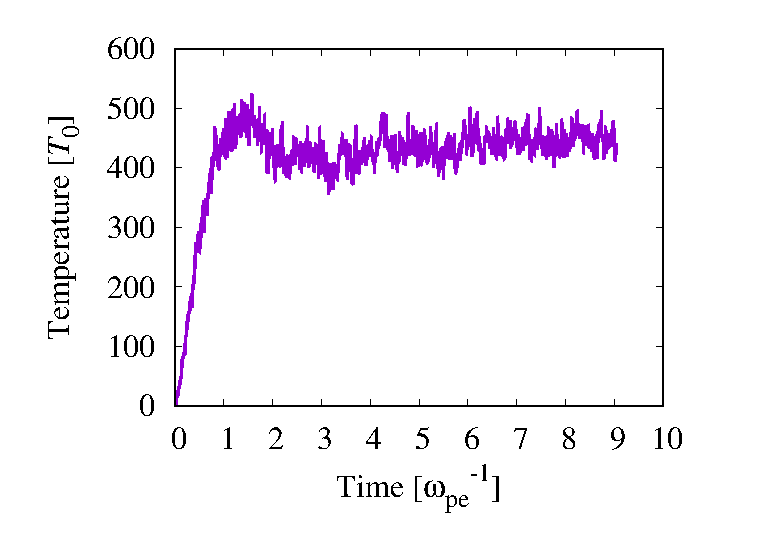
\includegraphics{numata01.eps}}
\caption{電子温度の時間変化.温度は$x$,$y$,$z$各方向でほぼ等しいため,
3方向の平均温度を取った.}
\label{numata01}
\end{center}
\end{figure}
平衡状態における系全体の平均電子温度は$T_{\mathrm{e}}^{sat}\approx440T_0$となった。
このとき電子のプラズマパラメタは$\Lambda_{\mathrm{e}}\approx10^3$,デバイ長は
$\lambda_{D\mathrm{e}}\approx0.23L$となる。
図\ref{numata02}に$y$方向の静電ポテンシャル分布を示す($x=0.5L$,$z=0.5L$とした)。
電子によるポテンシャルの遮蔽がよく再現できることが確認された(境界付近でのずれは,
サンプル粒子数が十分でないためであると思われる)。
\begin{figure}[h]
\begin{center}
\resizebox{7cm}{!}{\includegraphics{numata02.eps}}
\caption{静電ポテンシャルの空間分布。}
\label{numata02}
\end{center}
\end{figure}
ここでは,系の全エネルギーが一定のアンサンブルを考えているが,温度一定の
カノニカルアンサンブルを考えるほうが実際のプラズマとの比較がしやすい。
温度を一定に保つ熱浴の実装を検討している.
また,ここでは粒子数が$10^4$程度に留まり,FDPSの威力は十分発揮されている
とは言えないが,今後大規模計算を実施する際にその効果
を体感できることを期待している.

%%%%%%%%%%%%%%%%%%%%%%%%%%%%%%%%%%%%%%%%%%%%%%%%%%%
\subsection{プラズマの例2:純電子プラズマ実験に対応した2次元点渦シミュレーション}
本稿では,FDPSの開発チームより,2次元系の計算が正しく行えるか,チェッ
クを行って欲しい旨の依頼を受けたので,2次元点渦系シミュレーションが
FDPSで正しく実行できるか,試した。なお,点渦系は,モデルに内在する運
動論的効果により\cite{Yatsuyanagi2015b},現象を再現できる下限の粒子数
で行った場合の結果が,一番理にかなったものになるケースが多いため,
FDPSが得意とする多粒子,多並列でのシミュレーションを行う意味が薄い。
よって,本解説は,FDPSで2次元シミュレーションも作成できることを示すこ
とを第一目的とし,ベンチマーク結果は掲載しない。

2次元点渦シミュレーションでのターゲット物理系は,純電子プラズマ実験で
ある。
一般的なプラズマと異なり,電気的中性条件が破れたプラズマを非中性プ
ラズマとよび\cite{毛利2001},特に電子のみから構成される場合,純電子
プラズマとよぶ。軸方向に強磁場を掛けた真空容器内における磁場に垂直
な面内の電子のLarmor半径=0の極限での運動(案内中心近似)は$\vec{E}\times\vec{B}$
ドリフト運動となり,その時間発展方程式は2次元非圧縮流体方程式である
Euler方程式(正確には,回転微分をとった渦度方程式)で記述される\cite{際本2001-2}。
このとき,流れ関数がポテンシャル,渦度が電子数密度に比例する,という
関係が得られる\footnote{この関係の導出過程はベクトル解析のよい練習問題
なので,学生の皆さんはぜひチャレンジしてみてください。}。
この関係により,純電子プラズマ実験では電場と磁場により流体内部が制御
可能な流体実験を行うことができ,渦結晶に代表される自己組織化現象
を観測してきた\cite{Jin2000,Sanpei}。非粘性渦度方程式は,点渦法
で数値的に解くことが可能なため,筆者(Y.Y)は,純電子プラズマ実験で見
られる自己組織化現象とリンクした理論/シミュレーション研究を展開し
てきた。

2次元点渦系では,渦度方程式
\begin{equation}
	\frac{\partial \wz(\vr,t)}{\partial t} + \div(\wz(\vr,t) \vu(\vr,t)) =0
\end{equation}
の「形式的」解をDiracのデルタ関数$\delta(\vr)$で表現された点の集合体とする。
点の総数は$N$で表す。
\begin{equation}
	\wz(\vr,t) = \sum_{i=1}^N\Omega_i \delta(\vr - \vr_i)
\end{equation}
ここで$\wz(\vr,t)$は渦度,$\Omega_i$,$\vr_i$は$i$番目の点渦の強さを表す
循環,2次元位置ベクトルである。
点渦の時間発展は,離散化されたBiot-Savart積分となる。
\begin{align}
	\frac{d\vr_i}{dt} = & -\frac{1}{2\pi}\sum_{j=1(\neq i)}^N\Omega_i \frac{(\vr_i - \vr_j)\times\hat{\vec{z}}}{|\vr_i - \vr_j|^2}\notag\\
	& + -\frac{1}{2\pi}\sum_{j\neq i}\Omega_i \frac{(\vr_i - \bar{\vr}_j)\times\hat{\vec{z}}}{|\vr_i - \bar{\vr}_j|^2}\label{eqn:interaction}
\end{align}
右辺第2項は半径$R$の円形境界を表現する$\bar{\vr}_i = R^2\vr_i/|\vr_i|^2$
に置かれた鏡像渦からの影響を表す。

数値シミュレーションでは,適当な初期分布で$\vr_i$を初期化したあと,
相互作用(\ref{eqn:interaction})を計算する。今回は,分かりやすい例として,
Kelvin-Helmholtz(Diocotron)不安定性の計算を行った。結果を図に示す。
\begin{figure}[h]
\begin{center}
\resizebox{7cm}{!}{\includegraphics{yatsuyanagi01.eps}}
\caption{円形境界半径を1として,ドーナツの外側半径=0.8,内側半径=0.46,総粒子数=
4177,ドーナツの内部も点渦で満たされた円盤の剛体回転タイムスケール=10.8。}
\label{fig0}
\end{center}
\end{figure}
初期設定から求めた線形不安定モードは,不安定な順に2と3である\cite{Davidson2001}。
その中から,数値揺らぎにより,多くのエネルギーが蓄積されたモード3が
立ち上がっていると考えられる。また,$T=120,140$のプロットから,
境界をまたいで越境してしまう粒子がいないことから,円形境界も鏡像渦に
よって十分な制度で計算されていることがわかる。

紙面の残りを使って,今回,著者がつまずいた点,特にMPIに慣れていない
ことに由来する困難について述べてみたい。FDPSでは領域分割技法である
Tree法や,疎結合並列計算のためのAPIであるMPIに関する知識はまったく
必要ない。しかし,FDPS側でどのような内部処理を行っているのか,その
概要を理解していないと,どうにも解決できないバグを埋め込む結果とな
る\footnote{開発チームのみなさま,問題解決に協力して頂き,大変感謝
しております。}。粒子系におけるクーロン力の計算は,力を計算する場所
の粒子($i$粒子)それぞれについて,力の源泉となる粒子($j$粒子)から
の相互作用を計算する。このとき,非MPI環境下であれば,粒子に関連付け
られる添字の値が変化することはないので,同一粒子間の発散する相互作用
計算を回避する目的で,ループ内において$i\neq j$という条件が使用可能
である。しかし,FDPSの場合,各粒子の情報は時々刻々変化する位置に
応じて領域ごとに配分しなおされ,各MPIノードへ渡される$i$粒子の個数が
ほぼ一様になるような仕組みをもっている。このため,粒子の添字が
時々刻々変化するため,自己相互作用計算を排除する目的で$i \neq j$
という条件は使用できず。$i$粒子と$j$粒子の距離が0.0超か否かにより判定
することになる。指摘されてみれば当たり前の結論であるが,MPIでの
プログラミング経験がないと,障壁になりやすいと感じたので,敢えて
ここにtipsとして掲載した。
\section{おわりに}

本稿では、粒子系大規模並列化のためのフレームワーク FDPS を紹介しました。
現代の大規模計算では MPI 等での並列化が必須になっていますが、
FDPS を使うことでその部分は自分で開発しなくても、高性能な並列プログラ
ムを実現できます。本稿が読者の皆様の研究のためのプログラム開発の一助に
なれば
幸いです。

%\bibliographystyle{jjap}
%\bibliography{yatsuyanagi,numata}
\begin{thebibliography}{10}
\expandafter\ifx\csname url\endcsname\relax
  \def\url#1{\texttt{#1}}\fi
\expandafter\ifx\csname urlprefix\endcsname\relax\def\urlprefix{URL }\fi

\bibitem{numata1}
S.~Hamaguchi: J. Plasma Fusion Res. {\bf 78} (2002) 313.

\bibitem{numata2}
A.~P. et~al.: J. Plasma Phys. {\bf 84} (2018) 905840308.

\bibitem{numata3}
C.-P. Wang and Y.~Nishimura: IEEE Trans. Plasma Sci. {\bf 47} (2018) 1196.

\bibitem{numata4}
D.~F.~E. et~al.: Rev. Mod. Plasma Phys. {\bf 2} (2018) 9.

\bibitem{Yatsuyanagi2015b}
Y.~Yatsuyanagi and T.~Hatori: Fluid Dyn. Res. {\bf 47} (2015) 065506.

\bibitem{毛利2001}
毛利明博: プラズマ・核融合学会誌 {\bf 77} (2001) 213.

\bibitem{際本2001-2}
際本泰士: プラズマ・核融合学会誌 {\bf 77} (2001) 329.

\bibitem{Jin2000}
D.~Z. Jin and D.~H.~E. Dubin: Phys. Rev. Lett. {\bf 84} (2000) 1443.

\bibitem{Sanpei}
A.~Sanpei, Y.~Kiwamoto, K.~Ito and Y.~Soga: Phys. Rev. E {\bf 68} (2003)
  016404.

\bibitem{Davidson1990}
R.~C. Davidson: {\em Physics of nonneutral plasmas} (Addison-Wesley, Reading,
  1990) \SS 6.

\end{thebibliography}
\end{document}
